\subsubsection{RFID}
\label{subsubsec:RFID}

\paragraph{Problem}\mbox{}\\

Ein Bestandteil der Cocktailmaschine ist, mittles einem persönlichen kontaktlosen Chip oder Badge das Lieblingsgetränk auswählen zu können. Dazu wird auf die RFID\footnote{Radio-Frequency Identification}-Technologie gesetzt. Sie ermöglicht es mittels RFID-Tags oder auch mit NFC \footnote{Nead-Field-Communication} des Handys Daten zwischen Tag und Maschine auszutauschen. So kann der User identifiziert werden.

Damit die Datenübertragung stattfinden kann, wird an der Antenne ein Wechselfeld angelegt, welches im Folgenden Energiesignal genannt wird. Dieses induziert beim Empfänger eine Spannung, welche als Energieversorgung dient. Der Sender moduliert ein Datensignal über das Energiesignal. Die Informationen werden im Tag demoduliert und verwertet. Bei den Befehlen für den Tag geht es hauptsächlich um Lese- und Schreibmethoden. Bei einer Lesemethode des RFID wird ein Teil des Speichers abgefragt, bei Schreibmethoden wird der Speicher beschrieben.

\paragraph{Schaltungsaufbau}\mbox{}\\

Bild \ref{fig:Schema_RFID} zeigt den Schaltungsaufbau des RFID-Moduls. Darin ersichtlich sind folgende Teilbereiche:

\begin{itemize}
\item MFRC522 RFID IC
\item Antenne
\item Anpassnetzwerk für Antenne
\item Kommunikaitonsschnittstellen
\end{itemize}

\begin{figure}[!h]
\center
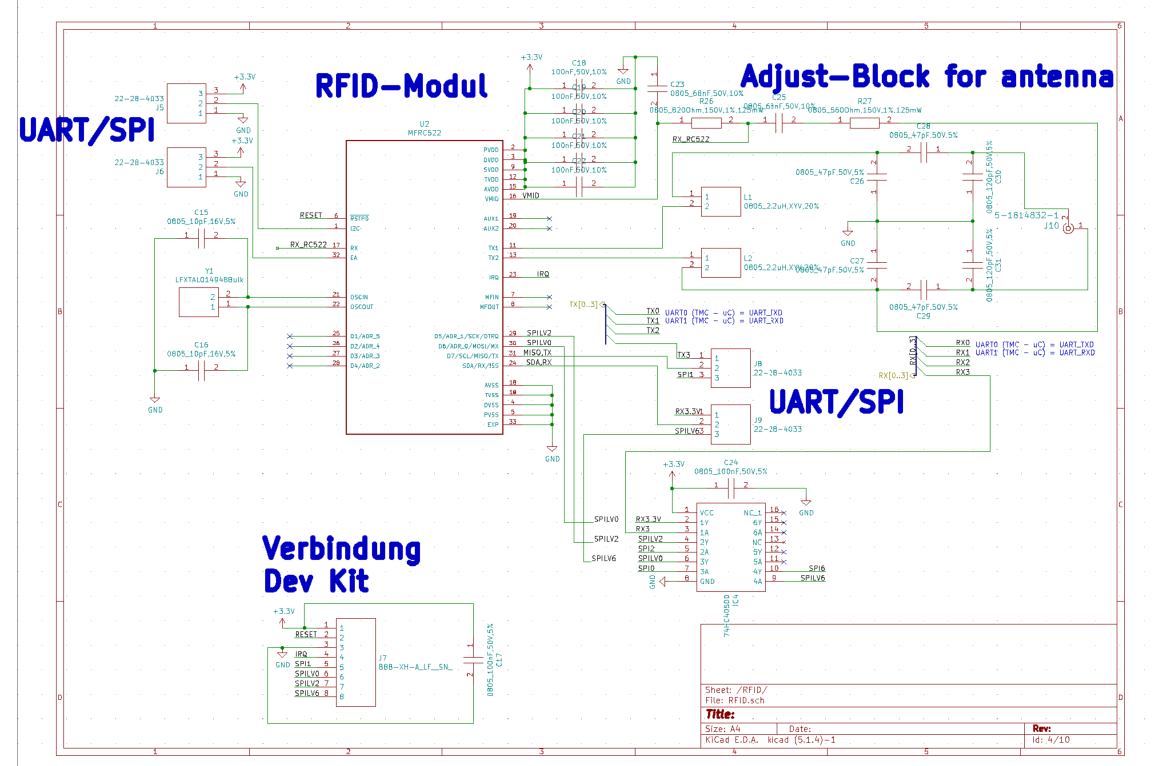
\includegraphics[width = \textwidth]{graphics/Schema_RFID}
\caption{Schema des RFID Sender/Empfänger}
\label{fig:Schema_RFID}
\end{figure}

\paragraph{Funktionsbeschrieb der Schaltung}\mbox{}\\

Der IC steuert den Ablauf, damit die Datenübertragung stattfinden kann. Er verbindet die Antenne mit dem System und wandelt die Informationen brauchbar von einer Seite auf die andere. Das Anpassnetzwerk sollte die gleiche Impedanz haben wie die Antenne. Wie die Bauteile dimensionert werden, kann in einer Anleitung nachgelsen werden. Sie dazu Anleitung: \cite{nxp_bv_2010_antenna_2010}.

Die Anschlüsse sind so gestaltet, dass falls eine einens gelayoutete Antenne verwendet wird, die Kommunikation zwischen UART und SPI gewählt werden kann. UART lässt sich einfacher in die Software einbinden, so die bisherige Erfahrung.

Für unser System wurde ein Breakout-Board verwendet. In erster Linie damit keine Zeit gebraucht wird, sich mit einem Antennendesign auseinandersetzen zu müssen. Aber auch, weil der IC in ein TQFP28-Gehäuse gepackt ist, und schwierigkeiten bereiten könnte beim Löten.